\documentclass{jarticle}
\usepackage[dvipdfmx]{graphicx}
\usepackage{here}
\usepackage{listings,jlisting} %日本語のコメントアウトをする場合jlistingが必要
%ここからソースコードの表示に関する設定
\lstset{
	basicstyle={\ttfamily},
		identifierstyle={\small},
		commentstyle={\smallitshape},
		keywordstyle={\small\bfseries},
		ndkeywordstyle={\small},
		stringstyle={\small\ttfamily},
		frame={tb},
		breaklines=true,
		columns=[l]{fullflexible},
		numbers=left,
		xrightmargin=0zw,
		xleftmargin=3zw,
		numberstyle={\scriptsize},
		stepnumber=1,
		numbersep=1zw,
		lineskip=-0.5ex
}
\title{ソフトウェア設計及び実験\\
	第6回レポート}
	\author{6119019056 山口力也}
	\date{2019/05/28日提出}


	\begin{document}
	\maketitle
	\section{原理}
	\subsection{サウンド処理}
	SDL2では,サウンドデータの種類にMusic型とChunk型の二つがある.以下にそれぞれの特徴を示す.
	\subsubsection{Music型}
	Music型には以下の特徴がある
	\begin{itemize}
	
	\item サウンドファイルのデータをメモリに全て読み込まず,ファイルからデコードしながら再生
	\item 同時に複数のMusic型サウンドは再生できない
		\begin{itemize}
		\item BGM(ある程度長いサウンド)再生に用いられる
		\end{itemize}
	\item Mix\_Music構造体(不透明構造体のためメンバは不明)
	\end{itemize}

	\subsubsection{Chunk型}
	Chunk型には以下の特徴がある.
	\begin{itemize}

	\item サウンドデータをメモリに読み込んで再生
		\begin{itemize} 
		\item 容量の小さいサウンドファイルを対象とすることが多い
		\end{itemize}
	\item 複数のサウンドを同時に再生できる
		\begin{itemize} 
		\item 効果音(即音声の高いサウンド再生)に用いられる
		\end{itemize}
	\item Mix\_Chunk構造体
	
	\end{itemize}

	\subsection{アニメーション処理}
	SDLでアニメーション処理を行う時は,いわゆるパラパラ漫画の要領で行う.複数の画像を用意し,一定時間間隔で次々に表示することによってアニメーション処理を実現できる.
	しかしながら,一定時間間隔で呼ぶ時,whileループの中で描画関数を呼び出すと,性能の低いCPUやプロセスが多く走っている場合アニメーションがゆっくりとなる可能性がある.また,Delay関数を入れると,その間に他の処理を行うことができない.その解決策はタイマー割り込みである.OSにより割り込みのタイミングが管理されているため,上記で述べた問題を解決できる.SDL2でのアニメーション処理の流れは以下の通りである.

	\begin{enumerate}
	\item キャラクタ画像や背景画像をサーフェイスに読み込む(IMG\_Load関数など)
	\item タイマーを設定,起動させる(SDL\_AddTimer関数)
	\item イベントループ(無限ループ)に入る
	\item 設定した時間間隔でコールバック関数が呼び出される
	\item 描画すべきキャラクタの動作パターンに対応する画像領域を抽出する
	\item 抽出した領域の画像データを描画対象(サーフェイスやレンダラー)に転送する
	\item 描画対象(レンダラー)をディスプレイに出力する
	\item 現在または次に抽出する画像領域を変数に格納する
	\item コールバック関数からイベントループに戻る
	\end{enumerate}

	\section{課題内容}
	オリジナルのアニメーションを作成せよ.
	\section{課題の結果}
	以下図\ref{fig:kadai1-1},図\ref{fig:kadai1-2},図\ref{fig:kadai1-3},図\ref{fig:kadai1-4}にアニメーションの結果画像を示す.

	\begin{figure}[H]
	\begin{center}
	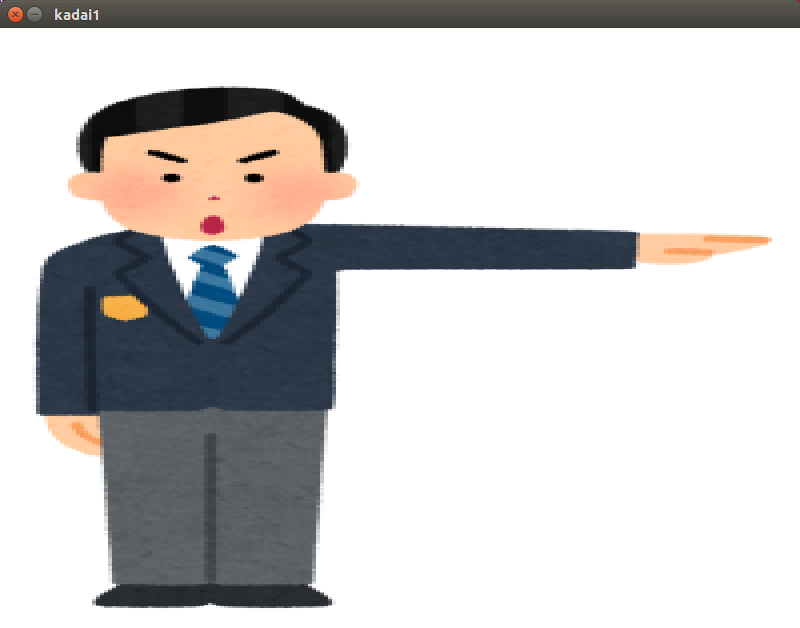
\includegraphics[width=7.0cm]{images/kadai1-1.png}
	\caption{課題1の出力画像の一例}
	\label{fig:kadai1-1}
	\end{center}
	\end{figure}


	\begin{figure}[H]
	\begin{center}
	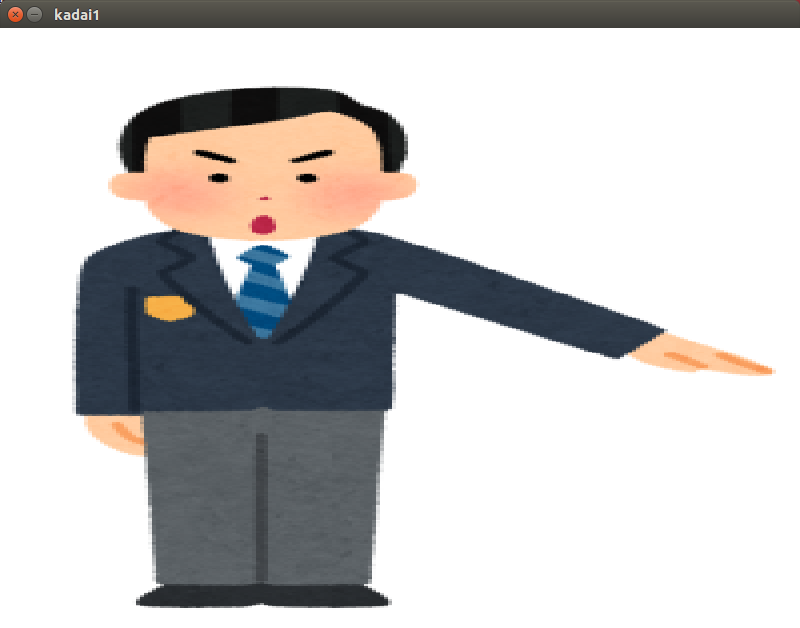
\includegraphics[width=7.0cm]{images/kadai1-2.png}
	\caption{課題1の出力画像の一例}
	\label{fig:kadai1-2}
	\end{center}
	\end{figure}


	\begin{figure}[H]
	\begin{center}
	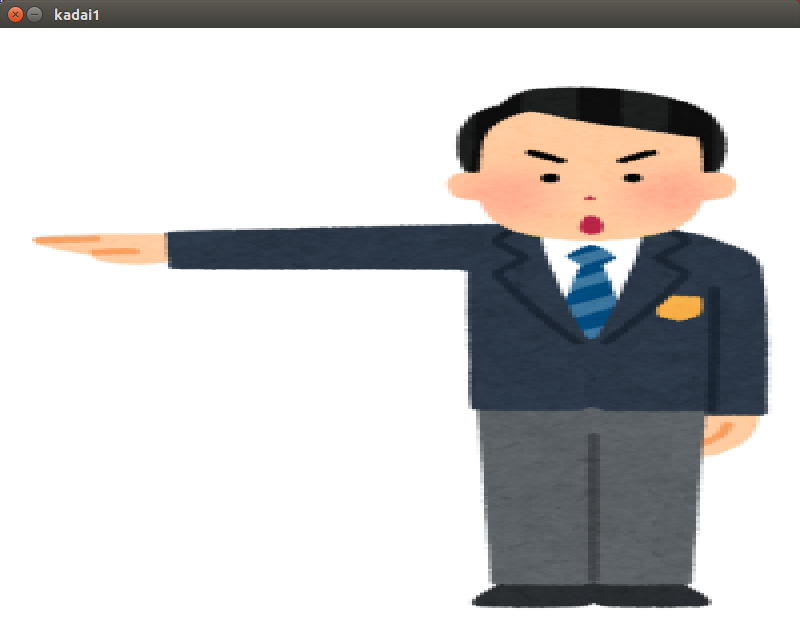
\includegraphics[width=7.0cm]{images/kadai1-3.png}
	\caption{課題1の出力画像の一例}
	\label{fig:kadai1-3}
	\end{center}
	\end{figure}


	\begin{figure}[H]
	\begin{center}
	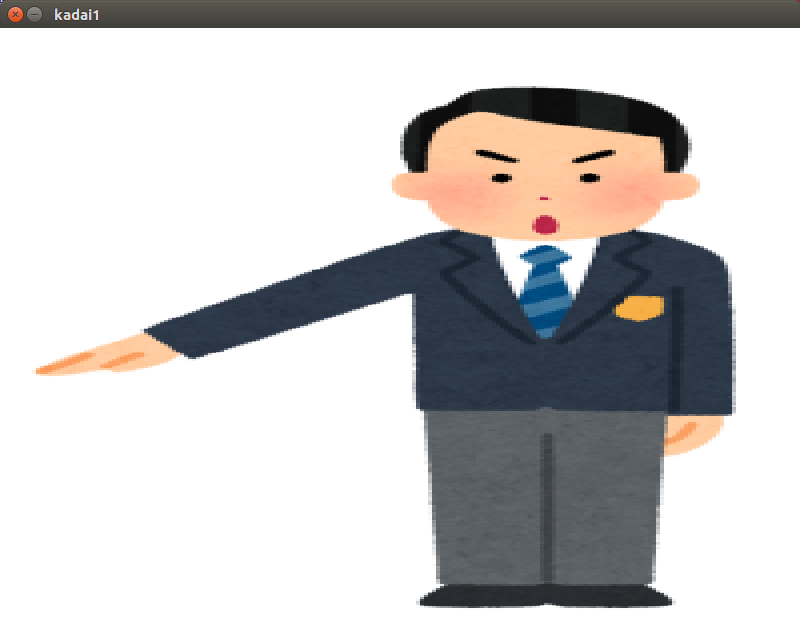
\includegraphics[width=7.0cm]{images/kadai1-4.png}
	\caption{課題1の出力画像の一例}
	\label{fig:kadai1-4}
	\end{center}
	\end{figure}

	\section{工夫した点}
	アニメーションをただ見るだけではつまらないので,BGMを付け加えた.BGMは2種類用意し,それぞれキーボードの"1"キーと"2"キーで切り替えれるようにした.BGMとしてはTELL(KATAMORI)とPerfect10(Unknown Brain,Heather Sommer)を用いた.TELLはFreeDownloadであったためCreative Commonsに従って使用する分には著作権には問題ないようであった.Perfect 10はNCS(No Copyright Sounds)であるためこちらも著作権には問題ないと思われる.
	\section{考察}
	アニメーションを行うときに画像をずらしていくが,ピクセルが少しでもずれていると描画対象がうまく写らない場合があった.そのため作成する画像の大きさ(ピクセル)には十分気をつけるべきだと思われる.また,アニメーションはタイマ割り込みの中で行われているため,呼び出す間隔には気をつけるべきだと思われる.実際タイマ割り込みの間隔を1msにすると処理が重すぎてPCが落ちてしまった.適当なタイミングでタイマ割り込みを行うことも大事な要素の一つだと思われる.
	\section{感想}
	今回の実験は前回に比べると簡単なものであったが,学んだことには,ゲームに必要な要素が多くあり,これから行うゲーム開発に欠かせない知識だと感じた.


\end{document}
